\chapter{The pipeline}
\label{chapter:the-pipeline}

In the introduction, we saw that during the last century, different but related speech technologies have been developed independently from each other. The major areas of research were about \acrfull{ASR} and \acrfull{TTS}. Following up shortly, \acrfull{NLG} and \acrfull{NLU} gradually gained interest. Finally, with the addition of the \acrfull{DM}, all those technologies have been gathered to construct a modular \acrfull{SDS}~\parencite{Jurafsky2000-intro-sds}. In this chapter, we describe briefly all the involved modules before focusing our attention on the \gls{DM}.

\section{A modular architecture}

\begin{figure}

    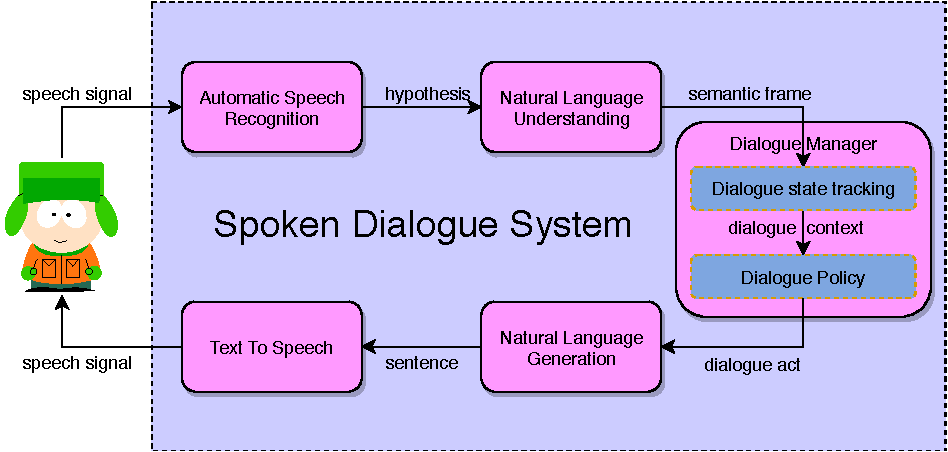
\includegraphics[width=\textwidth]{sources/pipeline/pipeline}
    \caption{\label{fig:pipeline} The architecture of a modular Spoken Dialogue System}
\end{figure}


\Cref{fig:pipeline} described the workflow leading a \gls{SDS}, processing a speech signal as an input and outputs an information of the same type.

\paragraph{Automatic Speech Recognition}

The \gls{ASR} module processes the speech signal. It produces interpretation hypotheses, as the most probable sentences the \idx{user} could have said. Each hypothesis is associated with a score we call the \gls{SRS}. As recalled in introduction, the state of the art of \gls{ASR} includes \acrlong{NN} solutions as for example the Connectionist Temporal Classification~\parencite{Kim2018-CTC-asr}, \gls{RNN}~\parencite{rnn-asr} and \gls{LSTM}~\parencite{Kim2017-lstm-asr}. They can also be combined with language modelling~\parencite{Chorowski2017-rnnml-asr,Kyungmin2018-rnnml-asr}.

\paragraph{Natural Language Understanding}

Given those hypotheses, the \gls{NLU} can extract meanings, and builds a \idx{semantic} frame corresponding to the last \idx{user} utterance, sometimes paired with a confidence score. Classic approaches parse the \idx{user} utterance into predefined \idx{handcrafted} \idx{semantic} slots~\parencite{chen2017-survey-sds}. Recent solutions are discriminated between two approaches. The first one considers using \glspl{NN}~\parencite{Deng2012-nn-for-nlu,Tr2012TowardsDU,Dauphin2014ZeroShotLA} or even Convolutional Neural Network~\parencite{Fukushima1980-cnn,Weng1993-cnn,LeCun1999-cnn} to directly classify the \idx{user} sentence from a set a pre-defined intents~\parencite{Hashemi2016QueryID,Huang:2013:cnn-intent-detection-nlu,Shen:2014:cnn-intent-detection-nlu}. The second one,  put a label on each word of the \idx{user}'s sentence. Deep Belief Networks~\parencite{Deng2012-nn-for-nlu} have been applied~\parencite{Sarikaya2011-deepbeleifnetwork-smeantic-tagger,Deoras2014-deepbeleifnetwork-smeantic-tagger}. \glspl{RNN} have been also used for \idx{slot-filling} \gls{NLU}~\parencite{mesnil2013-rnn-semantic-tagger,Yao2013-rnn-semantic-tagger-with-lm} and \gls{LSTM}~\parencite{Yao2014-lstm-semantic-tagger}. Some approaches consider bringing together \idx{user} intent and \idx{slot-filling}~\parencite{Zhang2016-joint-slot-filling-and-user-intent}.

\paragraph{Dialogue Manager}

By leveraging from the other modules, the \gls{DM} can decide the best thing to say, given the current state of the \idx{dialogue}. It is divided into two sub-modules, the \acrfull{DST}, and the \acrfull{DP}.

\subparagraph{Dialogue State Tracking}

The \gls{DST} keeps track of the history of the \idx{dialogue} (what the \idx{user} already asked, what slot is already filled, etc) and compiles it into a \idx{dialogue state} (could be called a belief state or also a \idx{dialogue} context, depending on the framework). It usually takes the form of confidence probabilities of each slot. Traditional approaches are rule-based~\parencite{Goddeau1996-handcrafted-dst,sadek1997artimis}. Statistical methods use Bayesian networks as recalled in ~\parencite{Thomson:2013-thesis-dialogue-management,Henderson-dst-review}. A recent approach is to consider merging \gls{NLU} and \gls{DST} into a single \gls{RNN}. The \idx{dialogue state} is then the hidden layer of a \gls{RNN} (or \gls{LSTM}) supposed to infer the next word in the \idx{dialogue}~\parencite{wen2017-rnn-hidden-state-for-mdp, barlier2018training}.

\subparagraph{Dialogue Policy}
The next step involves the \gls{DP}, extensively described in \Cref{sec:dm}, that chooses a \idx{dialogue act}~\parencite{austin1962,searle1969} according to the \idx{dialogue} context. The most simple form of \idx{dialogue act} is a parametric object used by the \gls{NLG} module to reconstruct a proper sentence. For example, if the domain of application is restaurant reservation, the \gls{DM} may ask for the area of the restaurant using the following \idx{dialogue act}: \texttt{request(slot=area)}\footnote{More details are provided in \Cref{sec:slot-filling-prob}}. In some recent work, the \gls{DP} actually outputs words~\parencite{li2016-dialogue-act-as-word,Vries2017-GuessWhat}. It seems natural to process this way, but that means the \gls{DM} must learn the \idx{semantic} of the language. Without proper metrics, it may lead to \glspl{DM} optimising the task with incoherent or ill-formed sentences.

\subparagraph{ }

It is worth noting that in the literature, \gls{DST} and \gls{DP} are not necessarily exposed as two distinct modules. For example, in ~\parencite{young2009-podmp-dst}, they cast the \gls{DST} and the \gls{DP} as a single \gls{POMDP}. The embedded Bayesian network of the \gls{POMDP} acts as the \gls{DST}.

\paragraph{Natural Language Generation}

The \gls{NLG} module would transcript the \idx{dialogue act} \texttt{request(slot=area)} as "Where do you want to eat?". Recently, \gls{LSTM} for \gls{NLG} has been used in the \gls{SDS} context~\parencite{lstm-nlg}.

\paragraph{Text To Speech}

Finally, the \gls{TTS} module transforms the sentence returned by the \gls{NLG} module into a speech signal. State-of-the-art approaches use generative models~\parencite{wavenet,Wang2017-TacotronTE-tts,Oord2018ParallelWF}.

\section{On the slot-filling problem}
\label{sec:slot-filling-prob}
In this thesis, we more specifically address \idx{slot-filling} \idx{dialogue} problems. For instance, we may consider an online form to book train tickets. The form contains several slots to fill, as for example birthdate, name, and address. The regular approach consists in filling each slot manually then send the HTML form to a server. This method exists for decades and has been used extensively on websites.
The advantage of this approach is that it is exact since forms include checkboxes and radio buttons and all other inputs are filled according to their labels (name, address, etc).
%
The counterpart is that the filling procedure may feel cumbersome to the \idx{user}. Interacting with the form directly through voice or chat instead of filling each slot may ease the process and this is the approach we consider. It involves a \gls{DS} asking the user the value of each slot in order to fill the form, then return the result of the form to the \idx{user}, partially or entirely, depending on the \idx{user} request. The \idx{user} experience is enhanced as the \idx{user} interacts in a natural fashion with the machine. Also, it can speed up the process as the \idx{user} can provide several slot values in a single utterance.

\subsection{Settings}

In order to describe the \idx{slot-filling} problem, we use a taxonomy similar to the \acrfull{DSTC} taxonomy~\parencite{dstc}. The problem is, for the system, to fill a set of slots (or goals). A slot is said \informable if the \idx{user} can provide a \textit{value} for, to use as a constraint on their search. A slot is said \requestable if the \idx{user} can ask the system the value of a slot.  All \informable slots are also \requestable. In the book train tickets example, the departure city is an \informable with a number of possible \textit{values} equal to the number of cities served by the transport. A non \informable slot, but \requestable, would be, for example, the identification number of the train.

\paragraph{User and system acts}

For purposes of conducting the \idx{dialogue}, the \idx{user} and the system are given respectively a set of user acts\index{user act} and system acts\index{system act}. Some acts are common to every dialogues\index{dialogue} such as \texttt{hello}, \texttt{repeat} or \texttt{bye}. Others acts depend on the ontology of the domain as they are direct instances of the \requestable and \informable slots. Both actors can request the value of a slot using the generic act \texttt{request(slot="a slot")} and inform the value of a slot using \texttt{inform(slot="a slot", value="its value")}. The counterpart of the \gls{DS} \idx{slot-filling} procedure is that an utterance may be misunderstood by the system. As the system is given an \gls{NLU} or \gls{NLU} score, it is able to judge if an utterance is worth asking for repeating. The system can ask the \idx{user} to repeat with several system acts:

\begin{itemize}
    \item \texttt{repeat}: the \idx{user} may repeat the last utterance. For instance "I don't understand what you said, please repeat.".
    \item \texttt{expl-conf(slot="a slot", value="its value")}: the system requests the \idx{user} to explicitly acknowledge a slot value. For example "You want to book a train departing from Paris, is it correct ?".
    \item \texttt{impl-conf(slot="a slot", value="its value")}: the system reports a slot value without explicitly asking the \idx{user} to confirm it. If the \idx{user} thinks the value is wrong, then he can decide to fix the mistake. For example "You want to book a train departing from Paris. Where do you want to go ?".
\end{itemize}

Note that, in \Cref{part:contributions-scaling} and \Cref{part:contributions-safe}, experiments will be conducted on \idx{slot-filling} problems with a similar taxonomy, but the acts may differ.


\section{The Dialogue Manager}
\label{sec:dm}

The particularity of the \gls{DM} as opposed to the other \gls{SDS}'s modules, is that it is stateful, in the sense that it needs to keep track of the \idx{dialogue state} to operate optimally\footnote{With modern approaches, any module using a \gls{RNN} may be also considered stateful.}. For example, we do not want to ask the same question twice if we have already got a clear answer. The \gls{DST} is stateful by definition but most of the time the \gls{DP} is stateless (it doesn't keep track of a state). This thesis proposes solutions to optimise the \gls{DM}.

Since the \gls{DM} is the only module involved, we abstract all the remaining modules into a single object called \idx{environment}. \Cref{fig:pipeline-dp} describes the simplified workflow: we assume the \gls{DM} to receive an object $o$ called the observation. It contains the last \idx{user} \idx{dialogue act} $a_{usr}$ (the \idx{semantic} frame) and the \gls{SRS}. We assume the \gls{DST} updates the next \idx{dialogue state} $s'$ given the current state $s$, the last \idx{system act} $a_{sys}$ and the last observation $o$. In this thesis, the \gls{DST} outputs a simple concatenation of the previous observations and \idx{system act}s. Also, we restrict the \idx{system act}s to \idx{dialogue act}s only (and not words).

\begin{figure}

    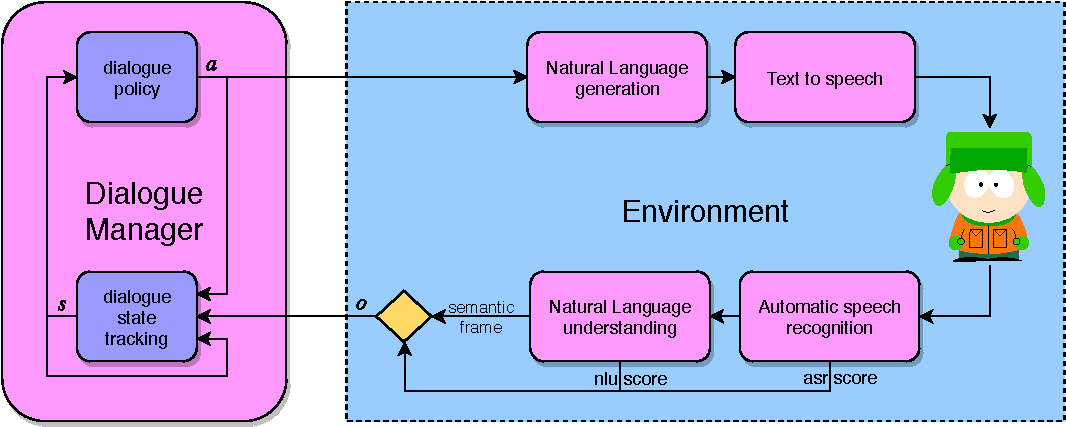
\includegraphics[width=\textwidth]{sources/pipeline/pipeline-dp}
    \caption{\label{fig:pipeline-dp} The pipeline view from the Dialogue Policy}
\end{figure}

Traditionally, \idx{handcrafted} approaches have been considered to design the \gls{DP}. They just match the \idx{dialogue state} to a \idx{dialogue act} using a set of \idx{handcrafted} rules for the \gls{DP}. It has been shown to be unreliable in unknown situations and it requires an expert knowledge on the domain. Statistical methods may solve these issues. Generative models have been considered to predict the next \idx{dialogue act} given the current state. This is typically how chit-chat bots work~\parencite{serban2016building,ijcai2018-778,Gao2018-neural-approches-convertional-ai}. State-of-the-art statistical approaches for \idx{task-oriented} \glspl{DS} involve \gls{RL}.


\paragraph{A Reinforcement Learning problem}

The previously cited methods do not really capture the sequential essence of a dialogue. By inferring the next \idx{dialogue act}, they just plan one step ahead. In order to plan multiple steps ahead, one can cast the \gls{DP} as a sequential decision making problem. \acrfullpl{MDP} are a good fit to mathematically describe those problems but they require a \idx{model} of the \idx{environment}. Unfortunately, it is not possible to get an analytic \idx{model} of the \idx{environment} since it involves human decision making. To overcome this issue, dialogue policies can be optimised using \acrfull{RL} algorithms, where the only prerequisite is having a dialogue corpus or the ability to directly interact with the \idx{user} in an \idx{Online} fashion.

